\subsection{Web Evolution}

In this section, we describe the evolution of the web, and introduce the
technologies that changed the way we browse today.



\subsubsection{Static HyperText Documents}
Upon its creation, the web was a system which consisted of only documents and links
connecting those documents. The request of a resource via  web browser
resulted in the retrieval of a static hypertext document over a network, which was
then rendered and presented to the user.





\subsubsection{Dynamically Generated Pages}
After a maturing period, the web evolved from a static file-page system,
into more complex web applications. The introduction of server side scripting languages
enabled web pages to be dynamically assembled on the fly. It also enabled access to
external applications, through the Common Gateway Inteface, CGI.
This made it possible to access databases, and use that information in the construction
of HTML documents.




\subsubsection{REST}
By the year 2000, the backbone of the web was well estabilished, and included
concepts such as HTTP, HTML and URI. These concepts were standardized
through the W3C, which also made recommendations about CSS and the Document
Object Model, DOM.
In addition to this, a new concept, called REpresentational State Transfer, REST,
was proposed by Fielding (2000), and largely adopted when building web services.
REST is an  architectural style used to  guide the design and development of
web applications.

In the web, resources can be acessed
by specifying a URL. REST is an extension of this concept, which provides
the guidelines necessary to design web resources in a scalable and consistent way.
REST is thus a convention on how to organize the resources that may be acessed by the client.




\subsection{Web 2.0}
The concept of Web 2.0 was introduced by O'Rilley, in 2005. This term is used to describe
the changing trends of web technology, in particular, the evolution
from static hyper-text read only systems into an era of dynamic user-created content,
and rich interactions between user and server.

This concept is ambiguously defined, but revolves around web techonologies that promote:

\begin{enumerate}
\item user as source of content - wikipedia project -
\item user collaboration and information sharing - social media
\item rich but simple interfaces - Google Maps -
\item software as a service - Google Docs
\end{enumerate}

Asynchronous JavaScript and XML, AJAX,
is the key technology that enables the rich content of the Web 2.0.


\subsection{AJAX}

In 1995, the Netscape 2 browser introduced the concept of Document Object Model, DOM.
DOM is a platform and language neutral model, for representing HTML and XML documents,
as a tree structure, where each node represents part of the document.
The DOM also provides an API to interact with the object. This allows the traversing
of such tree, or the update of content or stylying of the document or its parts.
Netscape also introduced a client-side scripting language, known as JavaScript.
Javascript was mostly used for updating the User Interface utilizing the DOM Api.
This technique was called Dynamic HTML.

In 1999, Microsoft introduced XMLHttpRequest, an API in the form of an object,
to transfer texts between web browser and web server. This API allows
various text formats, that invlude XML, HTML, plain text and JavaScript Object Notation, JSON.

In 2005, the term AJAX was proposed, and used to describe a set of technologies
that work together to permit the development of powerful web applications.
AJAX incorporates:

\begin{itemize}
\item standars-based presentation using XHTNL and CSS
\item dynamic display and interaction using the Document Object Model
\item data interchange and manipulation using XML and XSLT
\item asynchronous data retrieval using XMLHttpRequest
\item JavaScript binding everything together
\end{itemize}

The traditional model for web applications require some user action
to trigger an HTTP request, that is sent to the web server. The server
does some data processing, and then returns the HTML page to the client.
AJAX was proposed in order to create more responsive web applications,
and make asynchronous requests, that do not interfere with the display
of the existing pages. This generaly results in the decrease of the user felt latency.


An AJAX application has an intermediary between
the user and the server, the AJAX engine. In the start of a session,
instead of loading a web page, the browser loads an AJAX engine, written in javascript,
and usualy hidden away in some framework. This engine is responsible
rendering the web page, and communicating with the server on the users behalf.
The ajax engine allows the user interaction with the application
to happen asynchronously and independently from the communication with the web server.
Every user action that normally would generate an HTTP request, takes
the form of a javascript call to the Ajax engine instead. This engine
may then call the server in case it needs an external resource, or handles
the user action itself, if it has all the necessary data.
A comparison of the traditional model as oposed to the ajax one can be seen
in figure $\ref{fig:traditional_vs_ajax_model}$, while figure $\ref{fig:async_behaviour_ajax}$
illustrates the asynchronous behaviour of an AJAX application.

\begin{figure}
  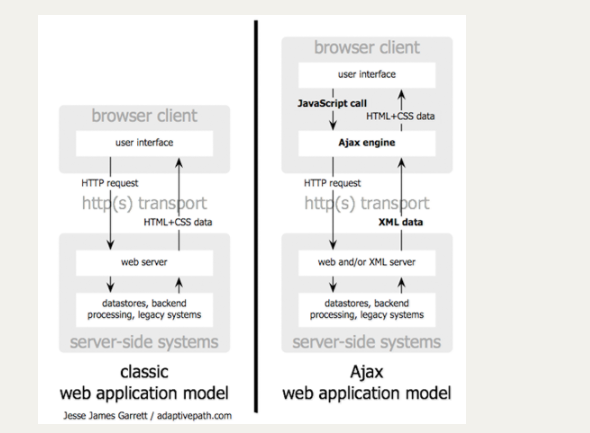
\includegraphics{Figures/web_services/traditional_vs_ajax_model}
  \caption{Two models for web applications, the traditional and the ajax models}
  \label{fig:traditional_vs_ajax_model}
\end{figure}

\begin{figure}
  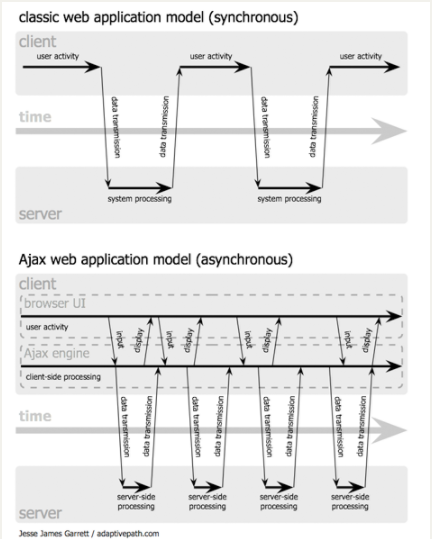
\includegraphics{Figures/web_services/async_behaviour_ajax}
  \caption{TThe synchronous interaction pattern of a traditional web application
  (top) compared with the asynchronous pattern of an Ajax application (bottom}
  \label{fig:async_behaviour_ajax}
\end{figure}
